\FloatBarrier
\chapter{Evaluation}
\label{sec:evaluation} 

\section{Evaluation Procedure}
The developed system was evaluated with four modeling experts to assess its usability and perceived usefulness, as well as to gather feedback on potential improvements and additional features. The evaluation process included a short demonstration, task-based activities, and a questionnaire. Each evaluation session lasted approximately 40 minutes.

The session was structured as follows: It began with a demonstration to introduce the tool's end-to-end workflow and key features. After that, the participants were asked to complete two tasks. The first was an exploratory task based on a fictional B2B order-processing scenario, consisting of two wiki-style documents\footnote{\url{https://github.com/ga94hor/doc-based-process-modeler/tree/evaluation_260324/evaluation_data/Task1_Fictional_B2BOrderProcessing}, accessed 2026-04-15} in DOCX format. It was designed to help participants familiarize themselves with the system. The second was a more realistic process modeling task based on an open-source SOP document\footnote{\url{https://dnrc.mt.gov/_docs/forestry/Wildfire/agreements-plans-guides/DNRC-Manuals/300-Fire-Business-Manual/Appendix-300-Manual/2023_Fire_Contract_PMT_SOP.pdf}, accessed 2026-04-15} in PDF format. For both tasks, participants were not given strict instructions on how to proceed, allowing them to explore the system freely. Due to the known issue of the PDF file rendering, the link to the online version was provided. If time permitted, participants could additionally use the system with their own documents. 

Following task completion, participants completed a questionnaire including the following open-ended questions: \\
(1) What aspects of the tool did you like while using it? \\
(2) What aspects of the tool did you not like or find problematic? \\
(3) What improvements or additional features would you most like to see in the tool? \\
(4) If you needed to model processes from documents in the future, would you consider using this tool? Why or why not?

\section{Evaluation Results}
\subsection{Overall Perception and Task Completion}
Overall, participants perceived the tool as usable and intuitive.  Figure ~\ref{fig:eva_expert2_task1} and Figure~\ref{fig:modeling-result-task2} show the modeling results from one expert for the first and second tasks, respectively. 

\begin{figure}[htb!]
    \centering
    \caption{Modeling result for Task 1} 
    % \floatfoot{Modeling result from an expert for the first task.}
    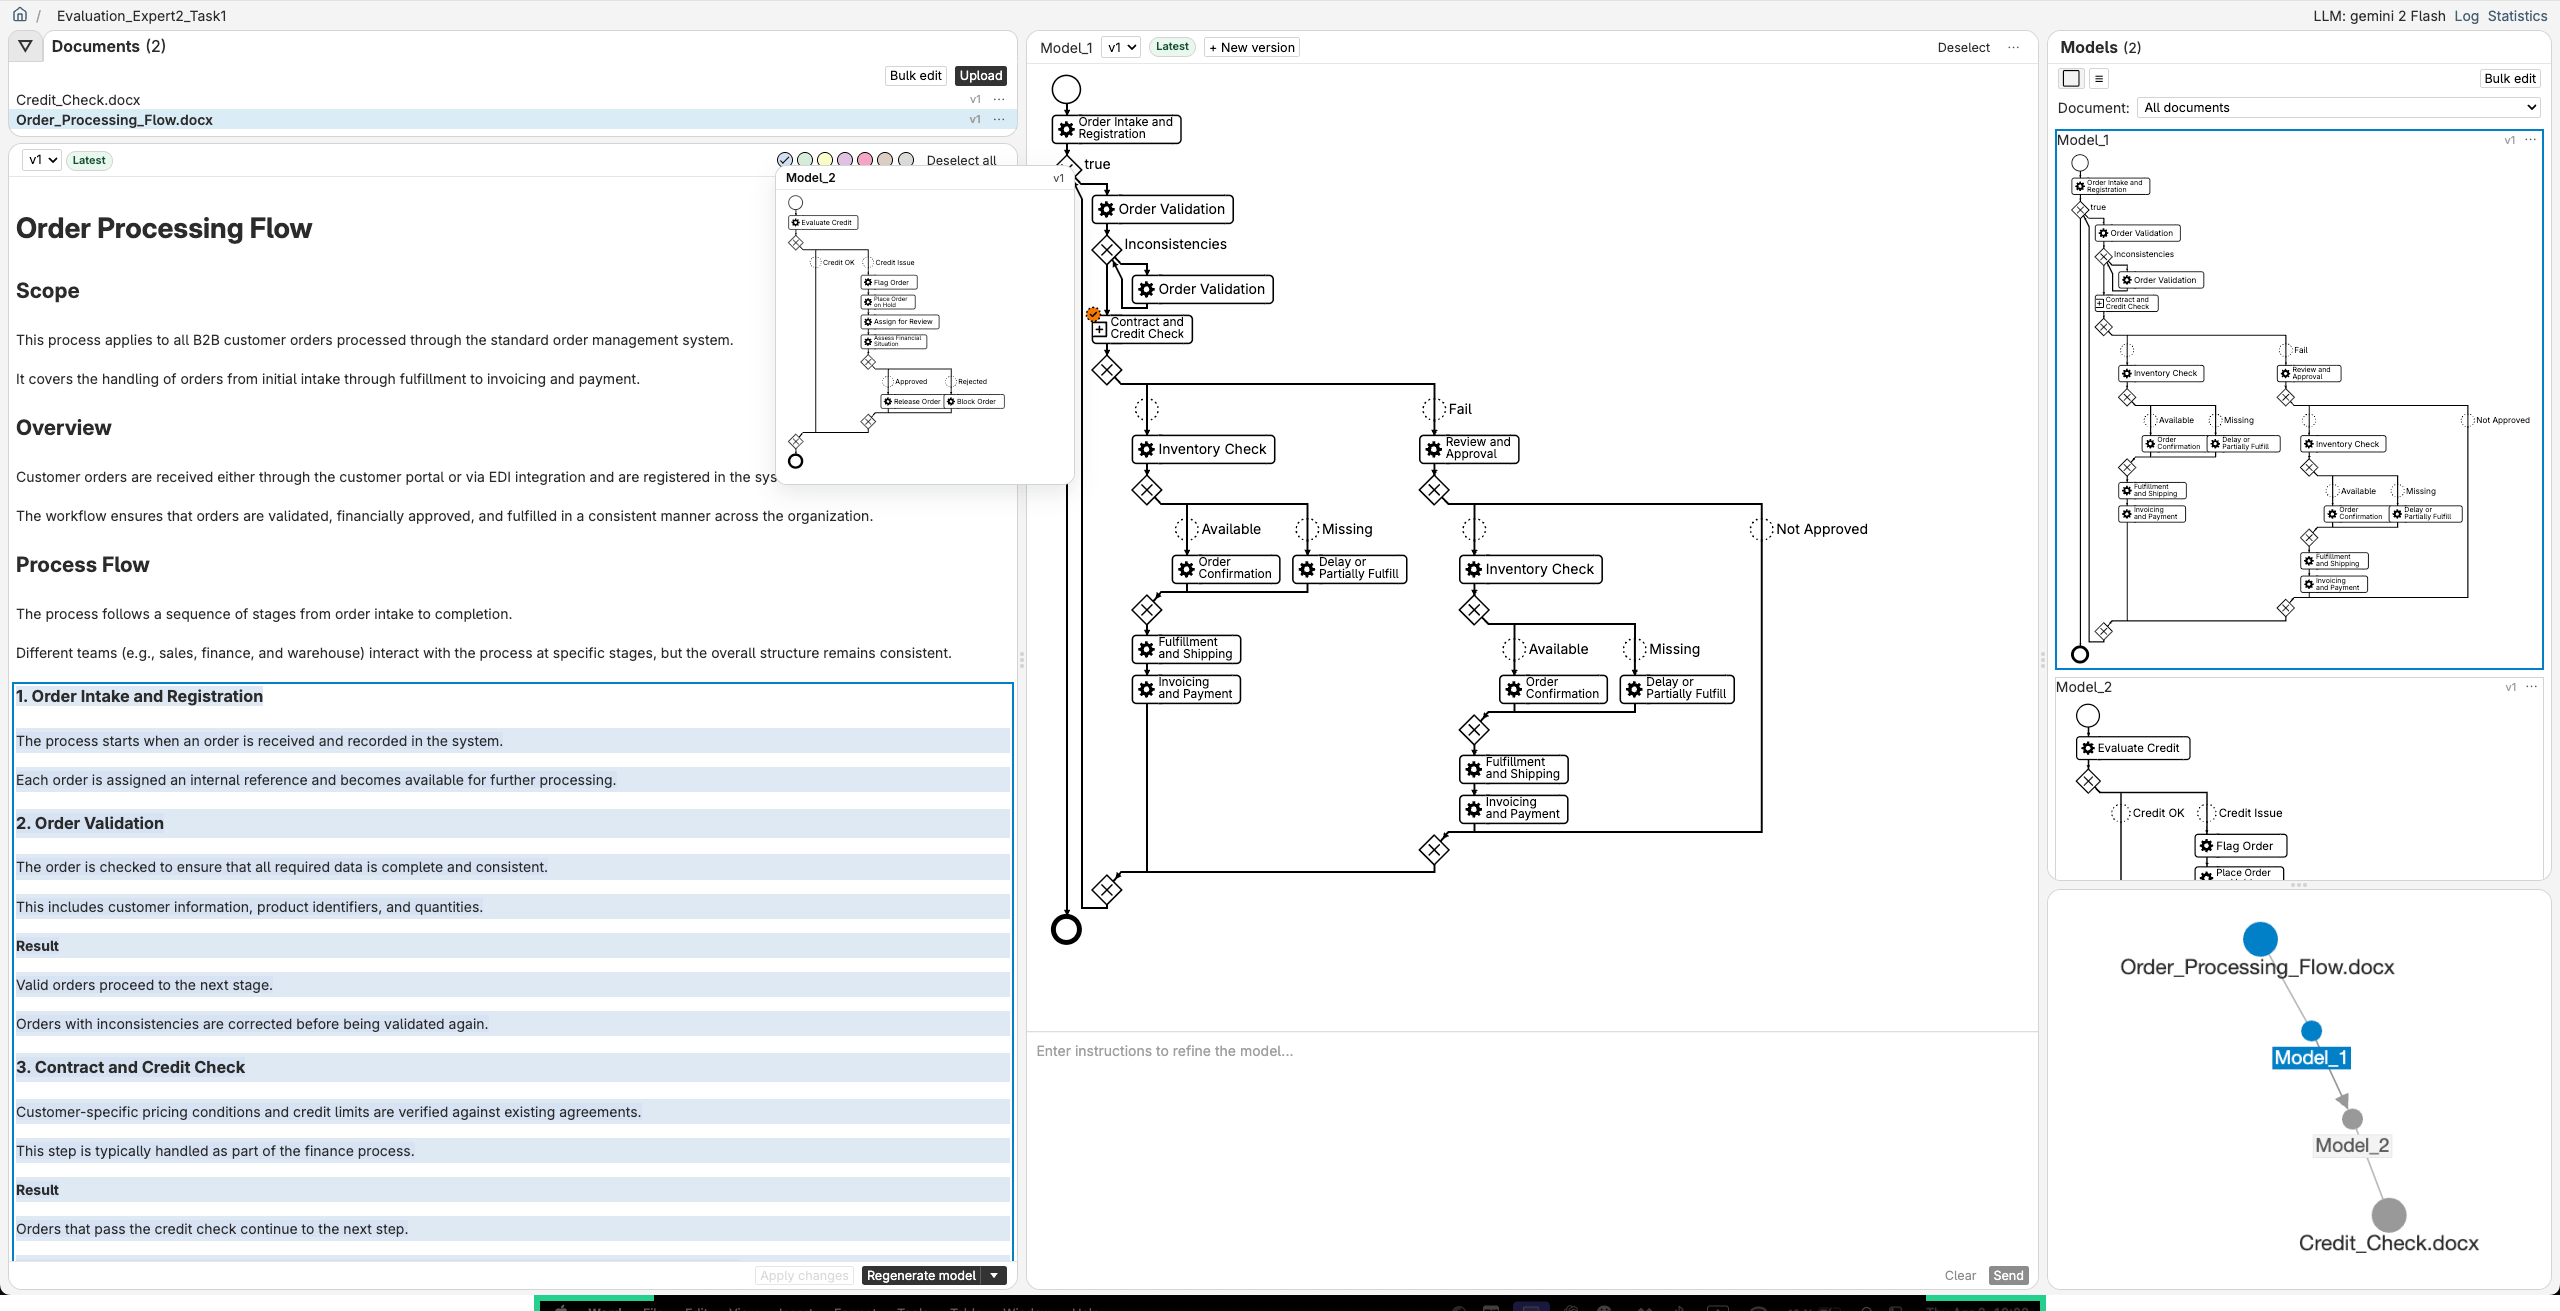
\includegraphics[width=1\textwidth]{images/eva_expert2_task1.png}
    \label{fig:eva_expert2_task1}
\end{figure}

\begin{figure}[htb!]
    \centering
    \caption{Modeling result for Task 2} 
% \floatfoot{Modeling result from an expert for the second task.}
    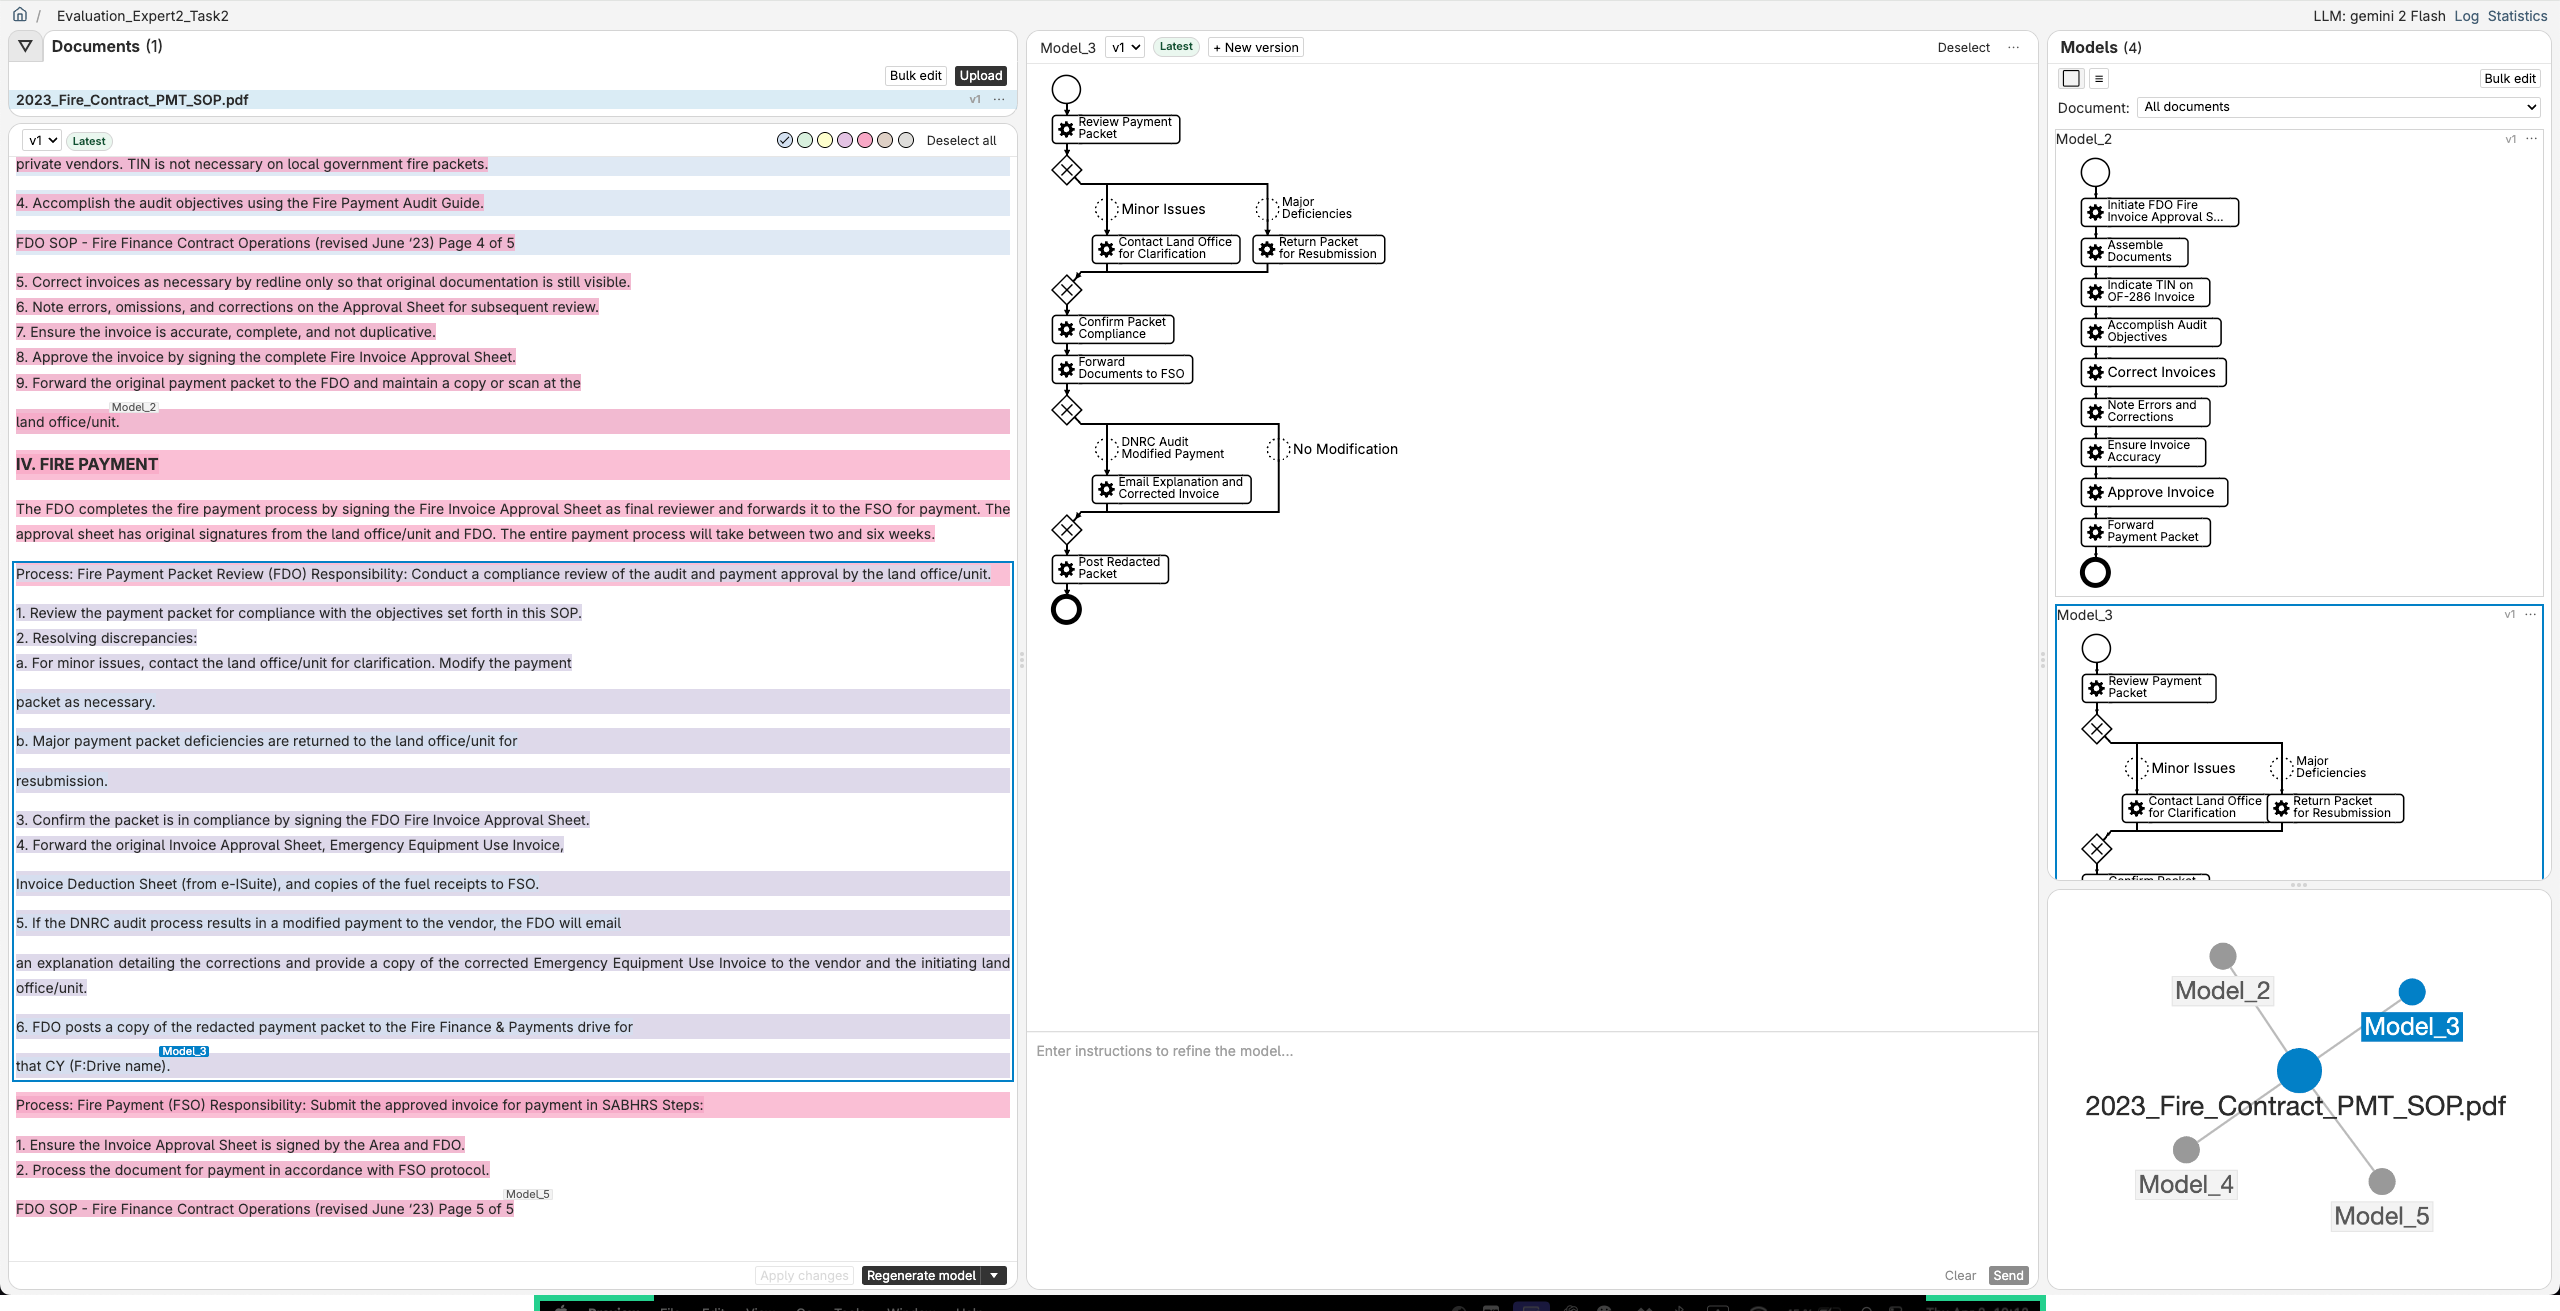
\includegraphics[width=1\textwidth]{images/eva_expert2_task2.png}
    \label{fig:modeling-result-task2}
\end{figure}

One interesting observation is that while most participants tended to start with, or at least try once, selecting larger portions or all of the text when reading a new document, one participant began by creating models from smaller segments. These different strategies are illustrated in Figure~\ref{fig:text-selection-strategies}.

\begin{figure}[htb!]
    \centering
    \caption{Different modeling strategies}
    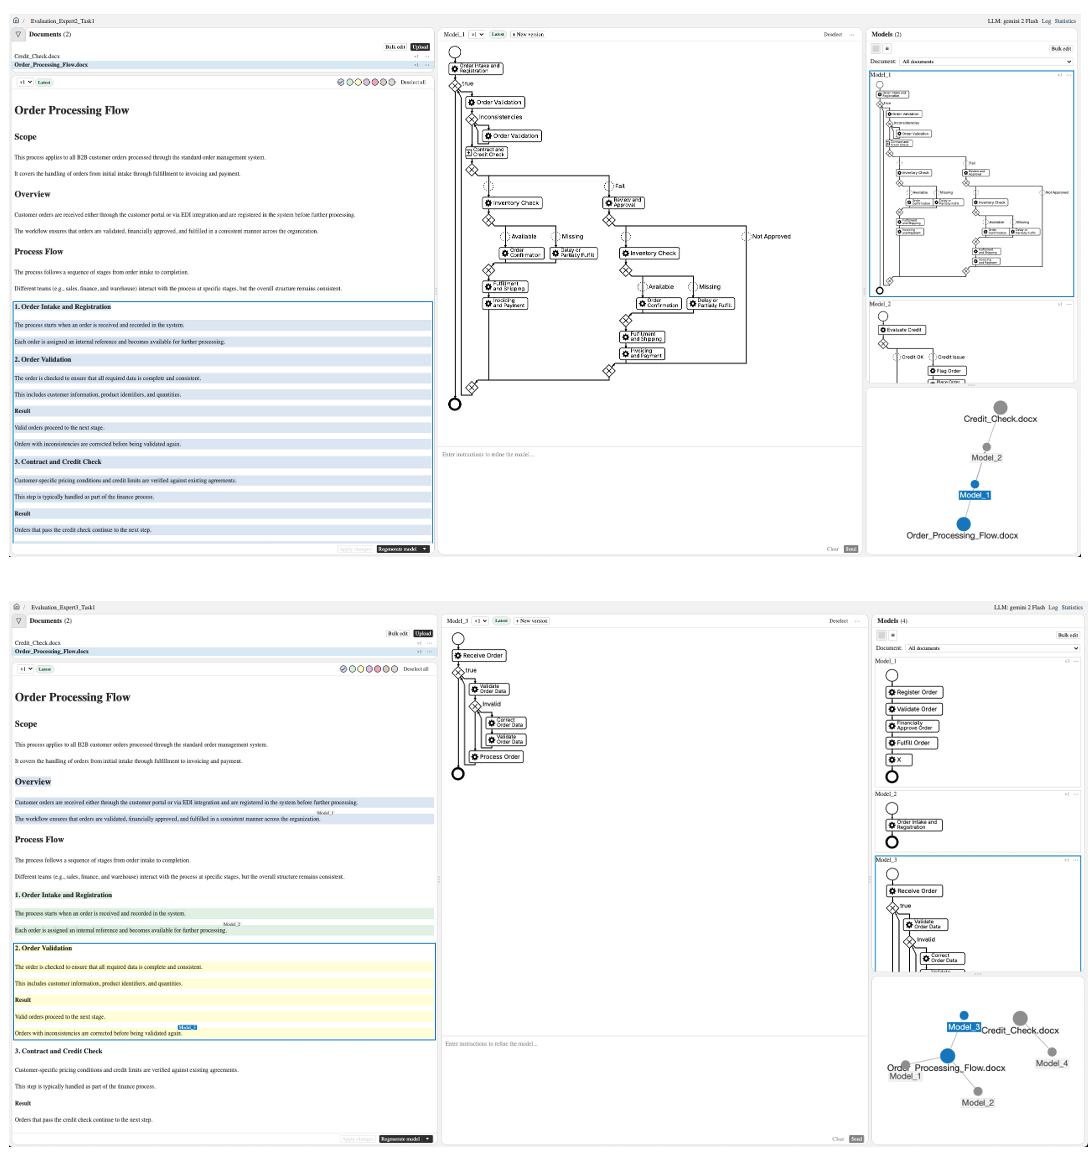
\includegraphics[width=0.7\textwidth]{images/Screenshot1.png}
    \floatfoot{Different modeling strategies observed during task execution (above: larger part selection; below: step-by-step selection)}
    \label{fig:text-selection-strategies}
\end{figure}

For detailed task completion and feedback, the participants showed varied interests and offered differing perspectives on the system. The result on each feature is summarized in Table ~\ref{table:evaluation-results}, and will be described in detail in the following sections. 

\begin{table}[htb!]
\centering
\caption{Summary of Evaluation Results by Functionality}
\floatfoot{n = number of participants who mentioned each item}
\label{table:evaluation-results}
\begin{tabular}{p{3cm} p{4cm} c p{4.5cm} c}
\toprule
\textbf{Functionality} & \multicolumn{2}{c}{\textbf{Positive Aspects}} & \multicolumn{2}{c}{\textbf{Problems and Limitations}} \\
\cmidrule(lr){2-3} \cmidrule(lr){4-5}
 & \textbf{Item} & \textbf{n} & \textbf{Item} & \textbf{n} \\
\midrule
\multirow{2}{3cm}{Document Rendering and Interaction}
& & & Readability issue  & 1 \\ 
\cmidrule(lr){4-5}
&  &  & Expected AI-assisted search capability & 1\\
\midrule
\multirow{2}{3cm}{Modeling Process}
& & & Unintuitive to start a new modeling by deselecting the current model & 2 \\ 
\cmidrule(lr){4-5}
&  &  & Unnecessary review step (of the initial generated model) & 2\\
\midrule
\multirow{2}{3cm}{Integrated LLM Service}
& Fast & 2 & Lack of transparency in the conversational modeling logic & 2 \\ 
\cmidrule(lr){2-3} 
& Good quality & 2 & & \\
\midrule
Model Versioning
& Helpful & 3 &  Expected version comparison & 1 \\
\midrule
Augmented Model Data
& Well-considered & 2 &  &  \\
\midrule
Text-Model Link & Clear & 1 & Expected fine-grained traceability & 2 \\
\midrule
Process-Subprocess Relationship
& Convenient & 3 &  &  \\
\midrule

\multirow{2}{3cm}{Project Graph}
& Helpful for larger systems & 1 & Unclear node types and version representations & 2 \\
\cmidrule(lr){4-5}
&  &  & Expected more expressive visualization & 1 \\
\midrule

Log and Statistics
& Potentially useful for analysis & 1 &  &  \\
\bottomrule
\end{tabular}
\end{table}

\subsection{Positive Aspects}
Firstly, the following aspects are generally perceived positively by the participants: the performance of the integrated LLM service, the easy-to-establish process-subprocess relationship, and model version control.

Furthermore, several additional positive aspects were mentioned. First, the embedding of relevant information, such as selected text and prompt history, within the model's XML data is considered a well-integrated design feature. Secondly, logging and statistical information elicited interest among some participants due to its potential for further analysis. Thirdly, the project graph visualization was mentioned as helpful, especially for larger systems.

\subsection{Problems in Interaction and Use}
The following outlines the main problems and challenges reported by participants, as well as notices observed during the evaluation.

First, for the document's rendering and interaction, only one feedback regarding the readability issue of PDF documents was mentioned in feedback. But it is observed that one participant started with reading the original PDF online firstly and one participant tried to use browser-extension to search for keywords.

Regarding the modeling process design, two problems were mentioned. First, the step to start a new modeling by a explicit deselection step of the current model was mentioned. Two reply received in the feedback, but it is a feature generally perceived as not intuitive immediately and needs additional clarification. Second, due to the sufficient good quality of the initial model, the review step was mentioned by one participant as totally unnecessary as there is version control and by another one as the initial generated model was mentioned as an unnecessary step.

Another main problem mentioned and observed is that the system's conventional modeling logic is not transparent to users and needs additional explanation. While the initial model generation from text was relatively clear, the model modification process was less transparent. They did not understand how their inputs were processed or how the system used the selected text and existing model. 
 
\subsection{Potential Improvements and Additional Features}
Besides the problems found during system use, many valuable insights were collected. 

For the existing features, improvements to the project graph visualization were mentioned most often. This includes clearer differentiation and identification of elements (i.e., what type of element a node is and which version it represents), as well as using more expressive visual designs, such as size, color saturation, and distance, to show additional information beyond type.

For document-related features, an AI-assisted document search and interaction function was suggested. This would allow users to query the document by providing an instruction, after which the retrieved parts can be automatically selected and used directly or as a basis for further adjustment for model generation.

For the process modeling features, one notable desired improvement emphasized by the participants is the need for finer-grained traceability between source text and model. When selecting larger text passages, only a subpart of the text is actually used and reflected in the generated model, and it is unclear which parts are actually used. Therefore, a clearer indication of the actual text used for model generation is required, ideally at the level of individual tasks. Secondly, model comparison was suggested as a valuable feature to help users understand and verify changes between different model versions, making it easier to identify modifications and track model iterations over time. Beyond this, participants also expected more general advanced AI modeling capabilities, including explainability of the generated model through conversational interaction with chatbots, as well as support for model quality evaluation and automatic improvement.

\subsection{Future Use Intention}
Three participants indicated an intention to use the system in scenarios involving the creation of multiple models. In such cases, the system’s features, such as text-model link, process-subprocess relationship, and model management functionalities, were considered helpful. One participant additionally raised the concern that automatically generated models may bypass the user’s need to fully understand the underlying document, potentially introducing bias. Hence, the fine-grained traceability, as suggested by the participant, could help mitigate this problem. Another participant again pointed out the need for the AI-assisted document search capability as suggested.



